\section{Deep Learning against Misalignment}
\begin{frame}
\frametitle{Contents}
\begin{itemize}
\item \textcolor{grey}{Introduction to LDA: as a classifier, and as a feature extractor
\item Introduction to masking countermeasure and Kernel Discriminant Analysis as a feature extractor}
\item \important{Convolutional Neural Networks and Data Augmentation to attack jitter-based countermeasure}
\end{itemize}
\end{frame}
\begin{frame}
\frametitle{Motivations to apply deep learning techniques}

\end{frame}

\begin{frame}
\frametitle{An integrated approach}
riprendi l'elenco puntato dell'inizio, barra tutto e dici che non si fanno più tanti step ma solo uno\\

più blocco che richiama il teorema di approssimazione universale
\end{frame}

\begin{frame}
\frametitle{Neural Networks}
schema a blocchi con tracce, split in training e validation, passa nel modello, funzione di costo, ottimizzo i pesi, monitoro, re-itero...tante volte..test
\end{frame}

\begin{frame}
\frametitle{Multi-Layer Perceptron}
le couche ...arrivare alla softmax richiamando la spiega sulla LDA

\end{frame}

\begin{frame}

\frametitle{Shift-invariance}
\end{frame}

\begin{frame}
\frametitle{Convolutional Neural Networks}
\end{frame}


\begin{frame}
\frametitle{Our CNN design principle}

\end{frame}


\subsection{Data Augmentation}
\begin{frame}
\frametitle{Data Augmentation}
\vspace{-11pt}
\begin{block}{Data Augmentation}
Artificially generate new training data by deforming those previously acquired,
Applying transformations that preserve the label $\sensRandVar$
\end{block}
\vspace{-5pt}
\begin{block}{Countermeasure Emulation Idea}
Emulate the effects of misaligning countermeasures to generate new traces
\begin{columns}
\begin{column}{0.35\textwidth}
\begin{large}
\textbf{\textcolor{green}{SHIFTING}}
\vspace{-8pt}
\end{large}
\end{column}
\begin{column}{0.35\textwidth}
\begin{large}
\textbf{\textcolor{blue}{ADD-REMOVE}}
\vspace{-8pt}
\end{large}
\end{column}
\end{columns}
\begin{figure}
  \begin{minipage}[b]{0.5\linewidth}
    \centering
    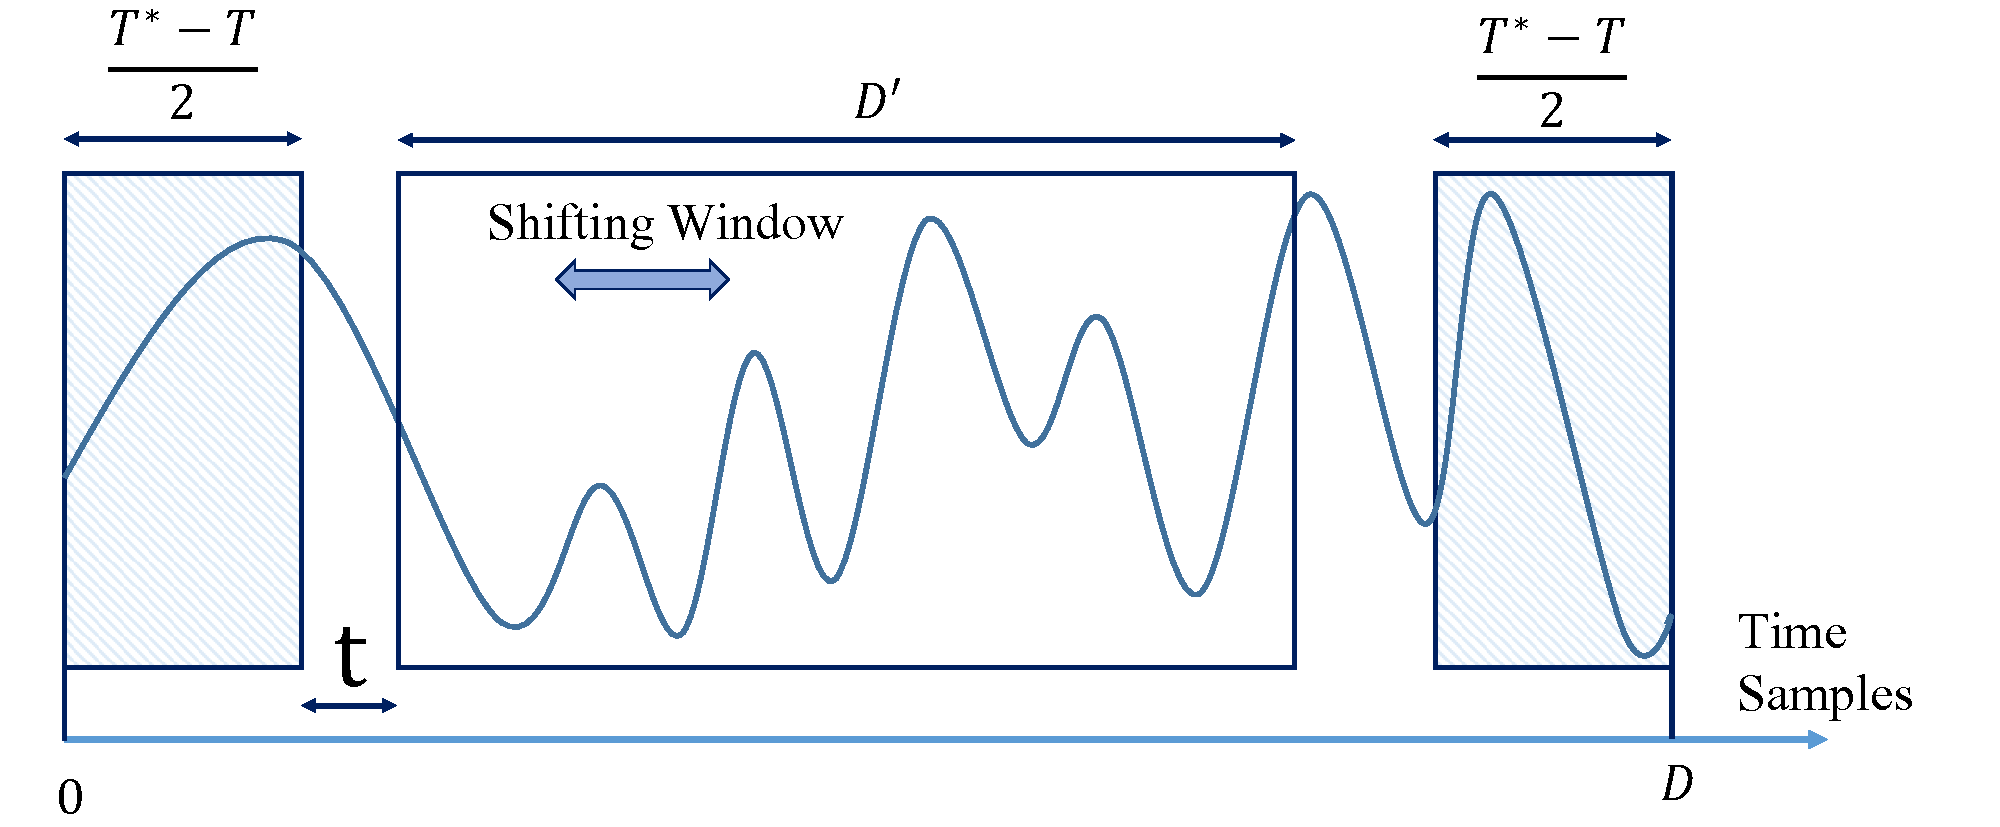
\includegraphics[width=\linewidth]{../Figures/CHES2017/Shifting_window.pdf} 
    \caption{\textcolor{green}{$SH_T$}}
  \end{minipage}%%
  \begin{minipage}[b]{0.5\linewidth}
    \centering
    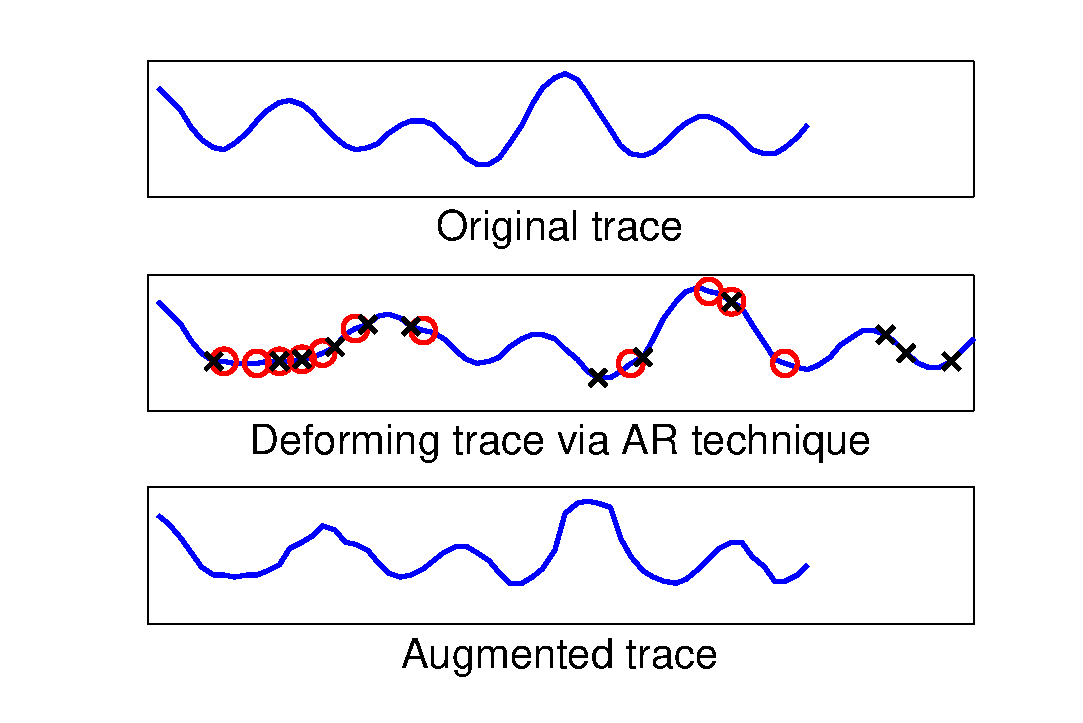
\includegraphics[width=.7\linewidth]{../Figures/CHES2017/AR_example.pdf} 
    \caption{\textcolor{blue}{$AR_R$}}
  \end{minipage} 
\end{figure}
\vspace{-9pt}
Parameter  \textcolor{green}{$T$}: $\sharp$ of possible positions \hfill \only<2->{\textcolor{red}{\small{$\longrightarrow$ new hyper-parameter}}}\\
Parameter \textcolor{blue}{$R$}: $\sharp$ of added and removed points \hfill \only<2->{\textcolor{red}{\small{$\longrightarrow$ new hyper-parameter}}}\\
Data Augmentation techniques are applied online during training phase.
\end{block}
\end{frame}


\subsection{Experimental Results}
\begin{frame}
\frametitle{Experimental Results}
\begin{itemize}
\item \only<1-2>{Random delays}\only<3>{\textcolor{red}{Random delays}}
\item \only<1-2>{Artificial Jitter}\only<3>{\textcolor{grey}{Artificial Jitter}}
\item \only<1-2>{Real Jitter}\only<3>{\textcolor{red}{Real Jitter}}
\end{itemize}
\uncover<2->{
\begin{block}{}
\begin{itemize}
\item Network architecture: 
$  \softmax \circ [\lambda]^1 \circ[\delta \circ [\sigma \circ \gamma  ]^1 ]^4$

\item Keras library with Tensorflow backend \cite{keras} (open source)
\end{itemize}
\end{block}
}
\end{frame}

\begin{frame}
\vspace*{-5pt}
\frametitle{Random delays}
\vspace{-18pt}
\begin{figure}
\subfloat[One leaking operation]{
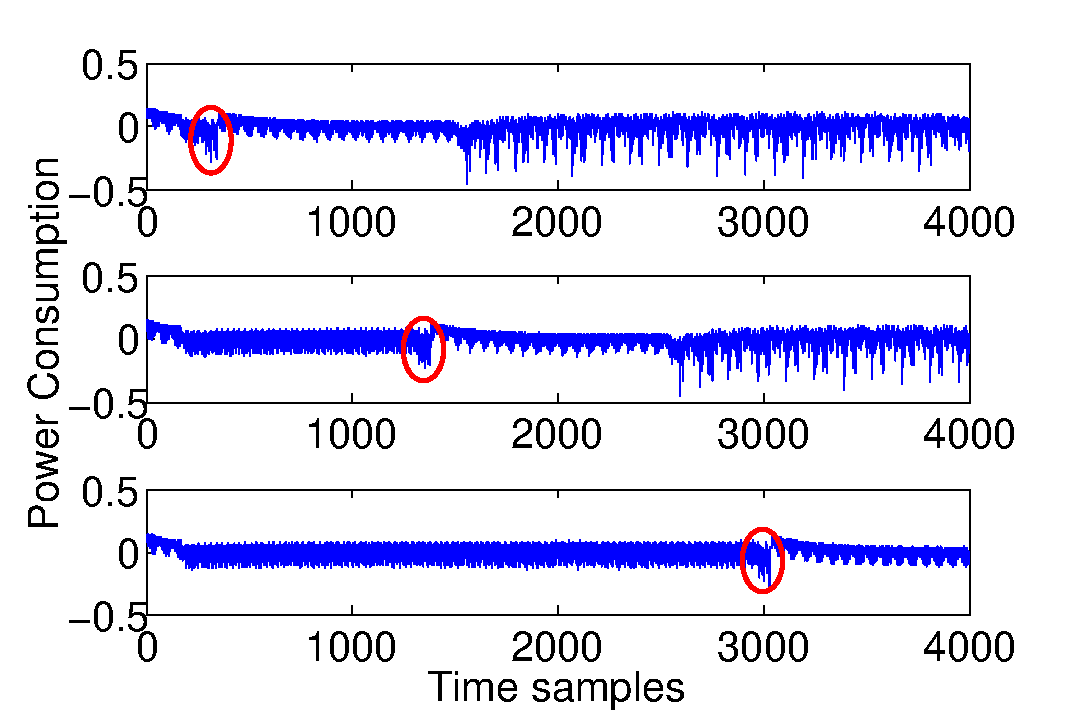
\includegraphics[width=.4\textwidth]{../Figures/CHES2017/CW_shift_traces.pdf} }

\end{figure}
\vspace*{-13pt}
\begin{block}{Setup}

\begin{itemize}
\item Target Chip: Atmega328P 
\item Target Variable: $Z = \mathrm{HW}(\mathrm{Sbox}(P\oplus K))$
\item Acquisition: through \emph{ChipWhisperer}\textregistered\ platform, $\approx 4,000$ time samples
\item Countermeasure: Random Delays - insertion of $r$ \emph{nop} operations, $r \in [0,127]$ uniform random
\item $1,000$ training traces

\end{itemize}
\end{block}


\end{frame}

\begin{frame}
\frametitle{Random delays}
\framesubtitle{Data augmentation vs overfitting}
\vspace{-8pt}
\begin{block}{Metrics}
\begin{itemize}
\item Test accuracy: classification accuracy over the attack traces
\item $N^\star$: minimum number of attack traces to make \emph{guessing entropy} of the right key permanently equal to one ($N^\star$ estimated over 10 independent attacks)
\end{itemize}
\end{block}


\begin{figure}
\captionsetup[subfigure]{labelformat=empty}
\subfloat[\textcolor{green}{$SH_0$}]{
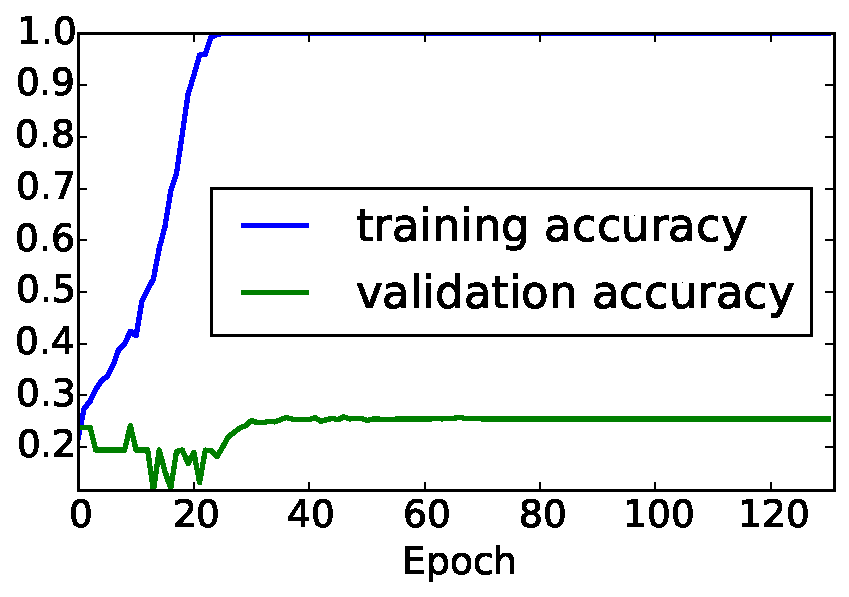
\includegraphics[width=.3\textwidth]{../Figures/CHES2017/DAshift0_2000traces_9classes_sgd/acc_DAshift0_2000traces_9classes_sgd.pdf} 
}
\subfloat[\textcolor{green}{$SH_{100}$}]{
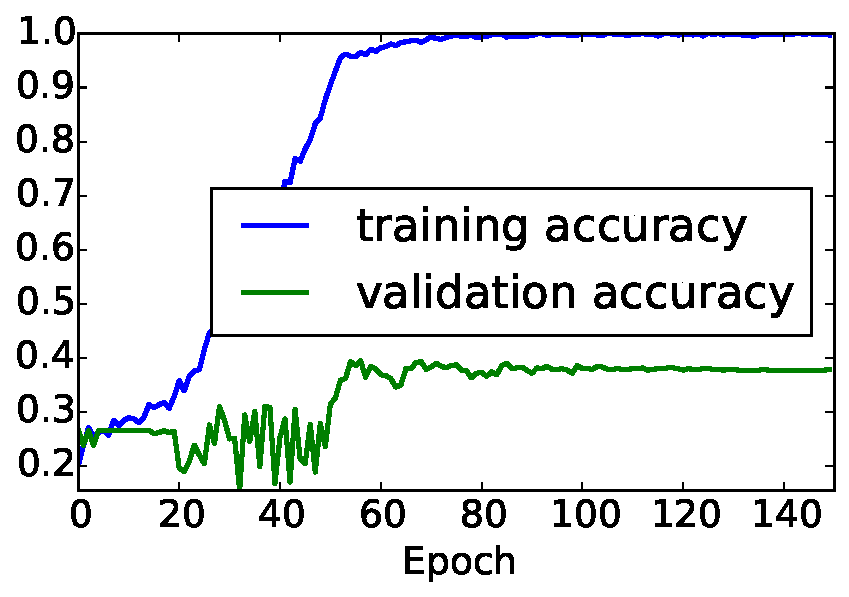
\includegraphics[width=.3\textwidth]{../Figures/CHES2017/DAshift100_2000traces_9classes_sgd/acc_DAshift100_2000traces_9classes_sgd.pdf} 
}
\subfloat[\textcolor{green}{$SH_{500}$}]{
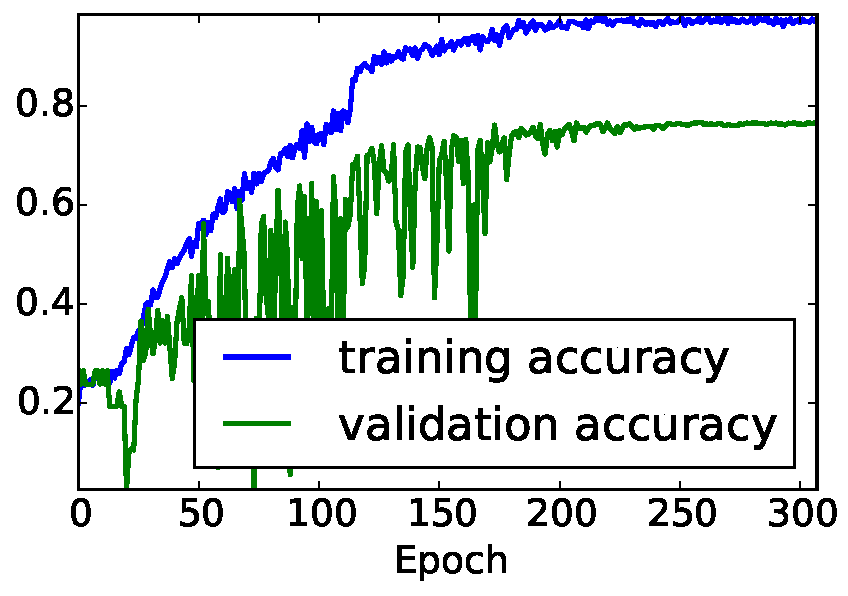
\includegraphics[width=.3\textwidth]{../Figures/CHES2017/DAshift500_2000traces_9classes_sgd/acc_DAshift500_2000traces_9classes_sgd.pdf} 
}
\end{figure}

\pause
\vspace*{-15pt}
\begin{table}
\begin{tabular}{|c|c|c|c|c|c|c|c|}
\multicolumn{8}{c}{}\\
\hline
\multicolumn{2}{|c|}{} & \multicolumn{2}{c|}{\textcolor{green}{$\mathrm{SH}_{0}$}} & \multicolumn{2}{c|}{\textcolor{green}{$\mathrm{SH}_{100}$}} & \multicolumn{2}{c|}{\textcolor{green}{$\mathrm{SH}_{500}$}} \\ \hline
Acc        & $N^\star$       & 27.0\%                      & $>1,000$                      & 31.8\%                       & 101                         & \textbf{78\%}              & \textbf{7}                \\ \hline
\end{tabular}
\end{table}
%
\end{frame}
%

\begin{frame}
\frametitle{Random Delays - Two Leaking Operations}

\centering
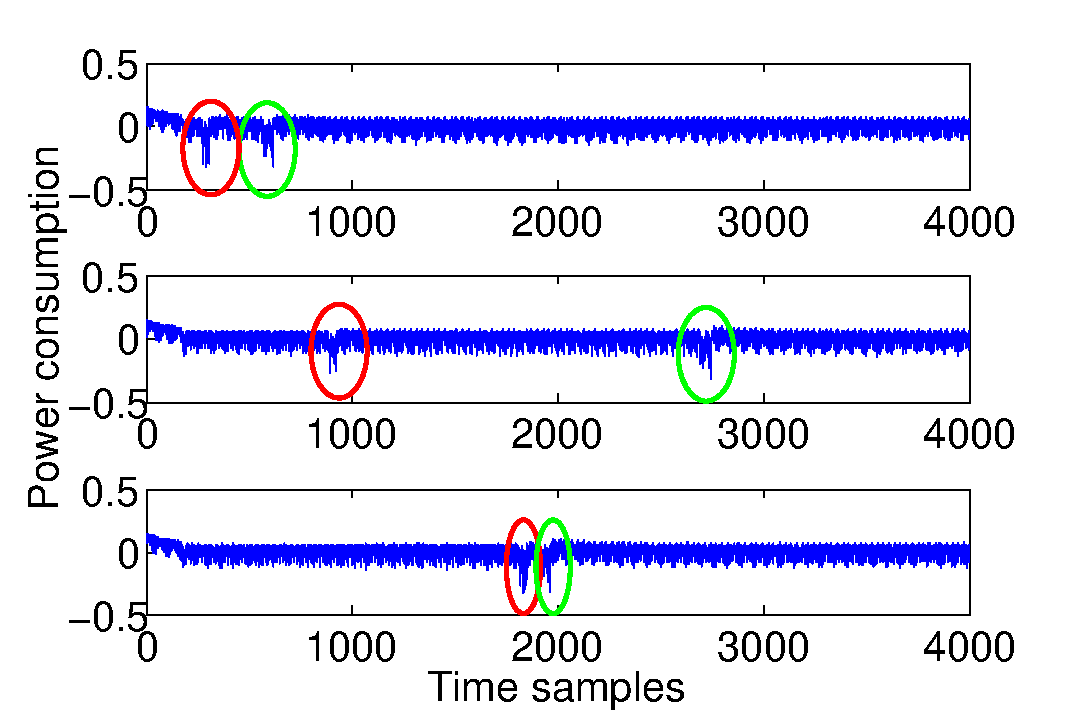
\includegraphics[width=.5\textwidth]{../Figures/CHES2017/CW_double_shift_traces.pdf}	


\begin{block}{Two leaking operations}
First operation - Test acc: $76.8\%$, $N^\star=7$\\
Second operation - Test acc: $82.5\%$, $N^\star=6$
\end{block}

\end{frame}

\begin{frame}
\frametitle{Artificial Jitter}
\begin{figure}
\subfloat[Low artificial jitter]{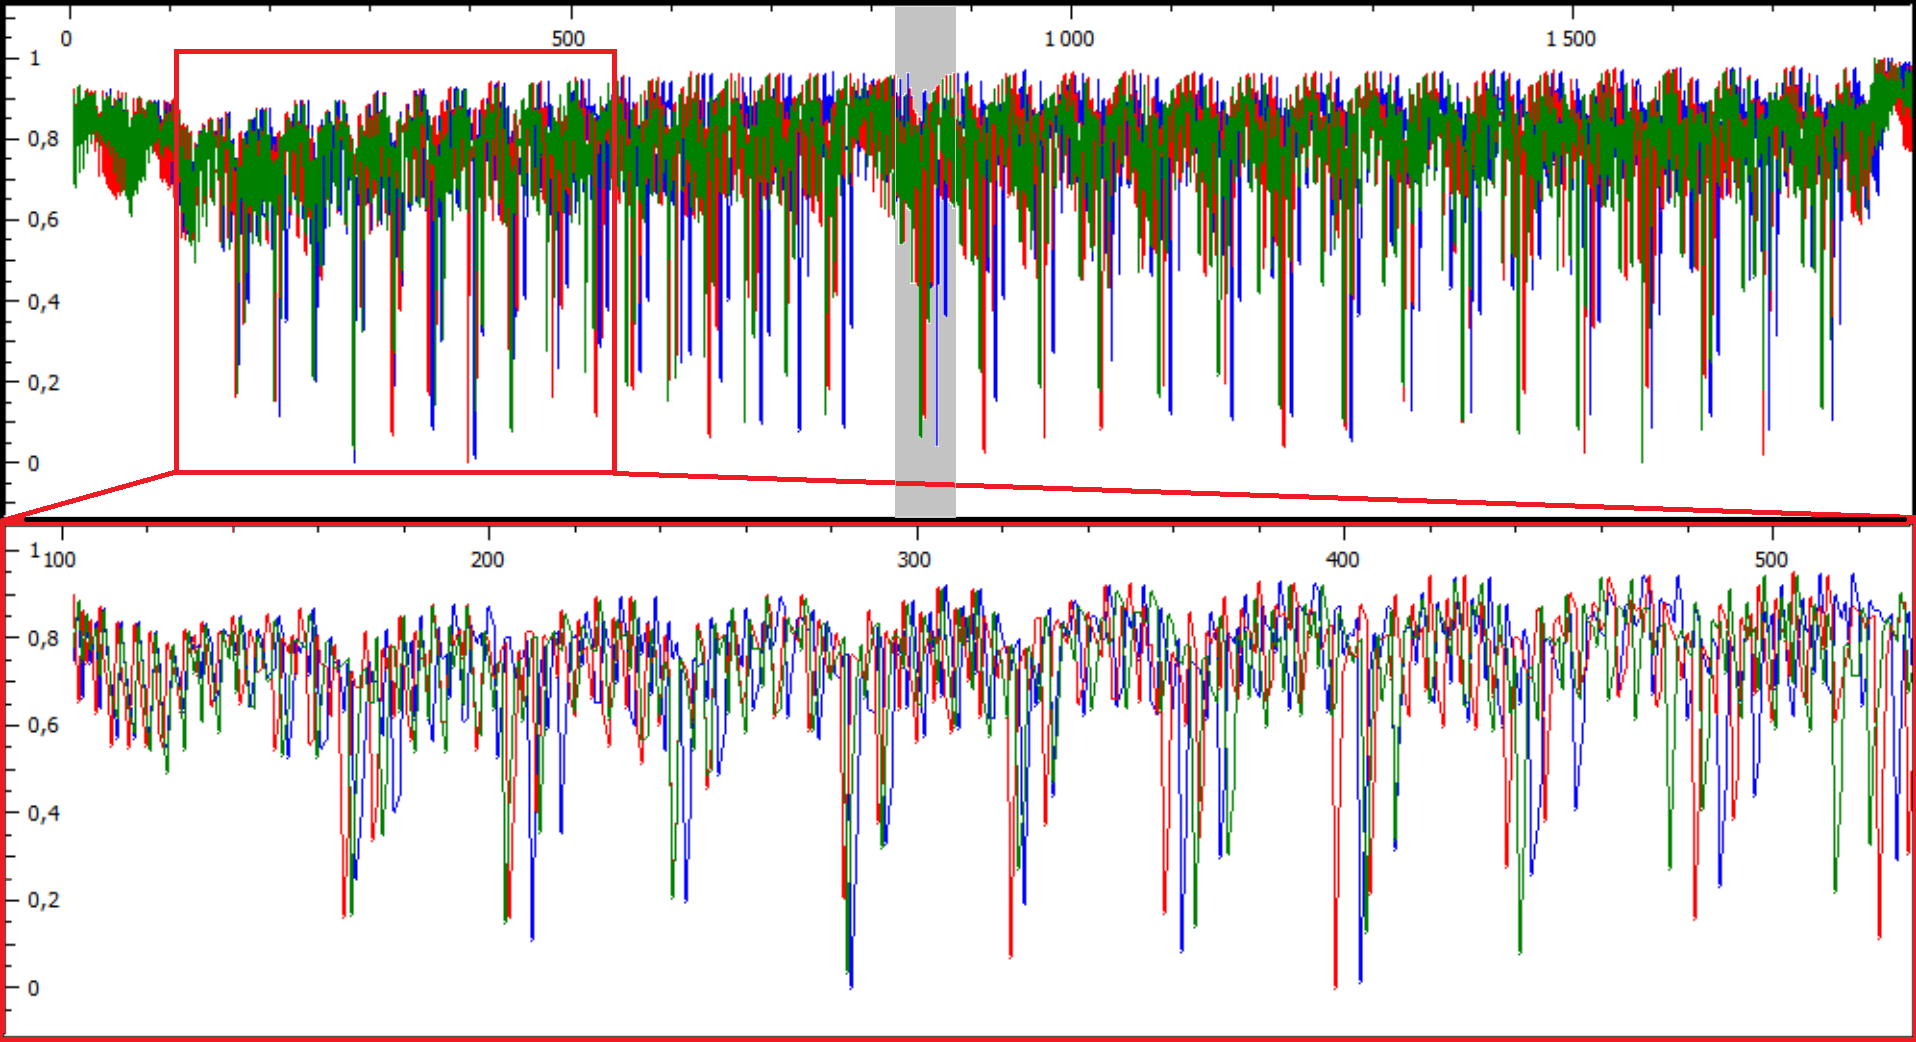
\includegraphics[width=.4\textwidth]{../Figures/CHES2017/jitter_2_2_framed.png} }
\subfloat[High artificial jitter]{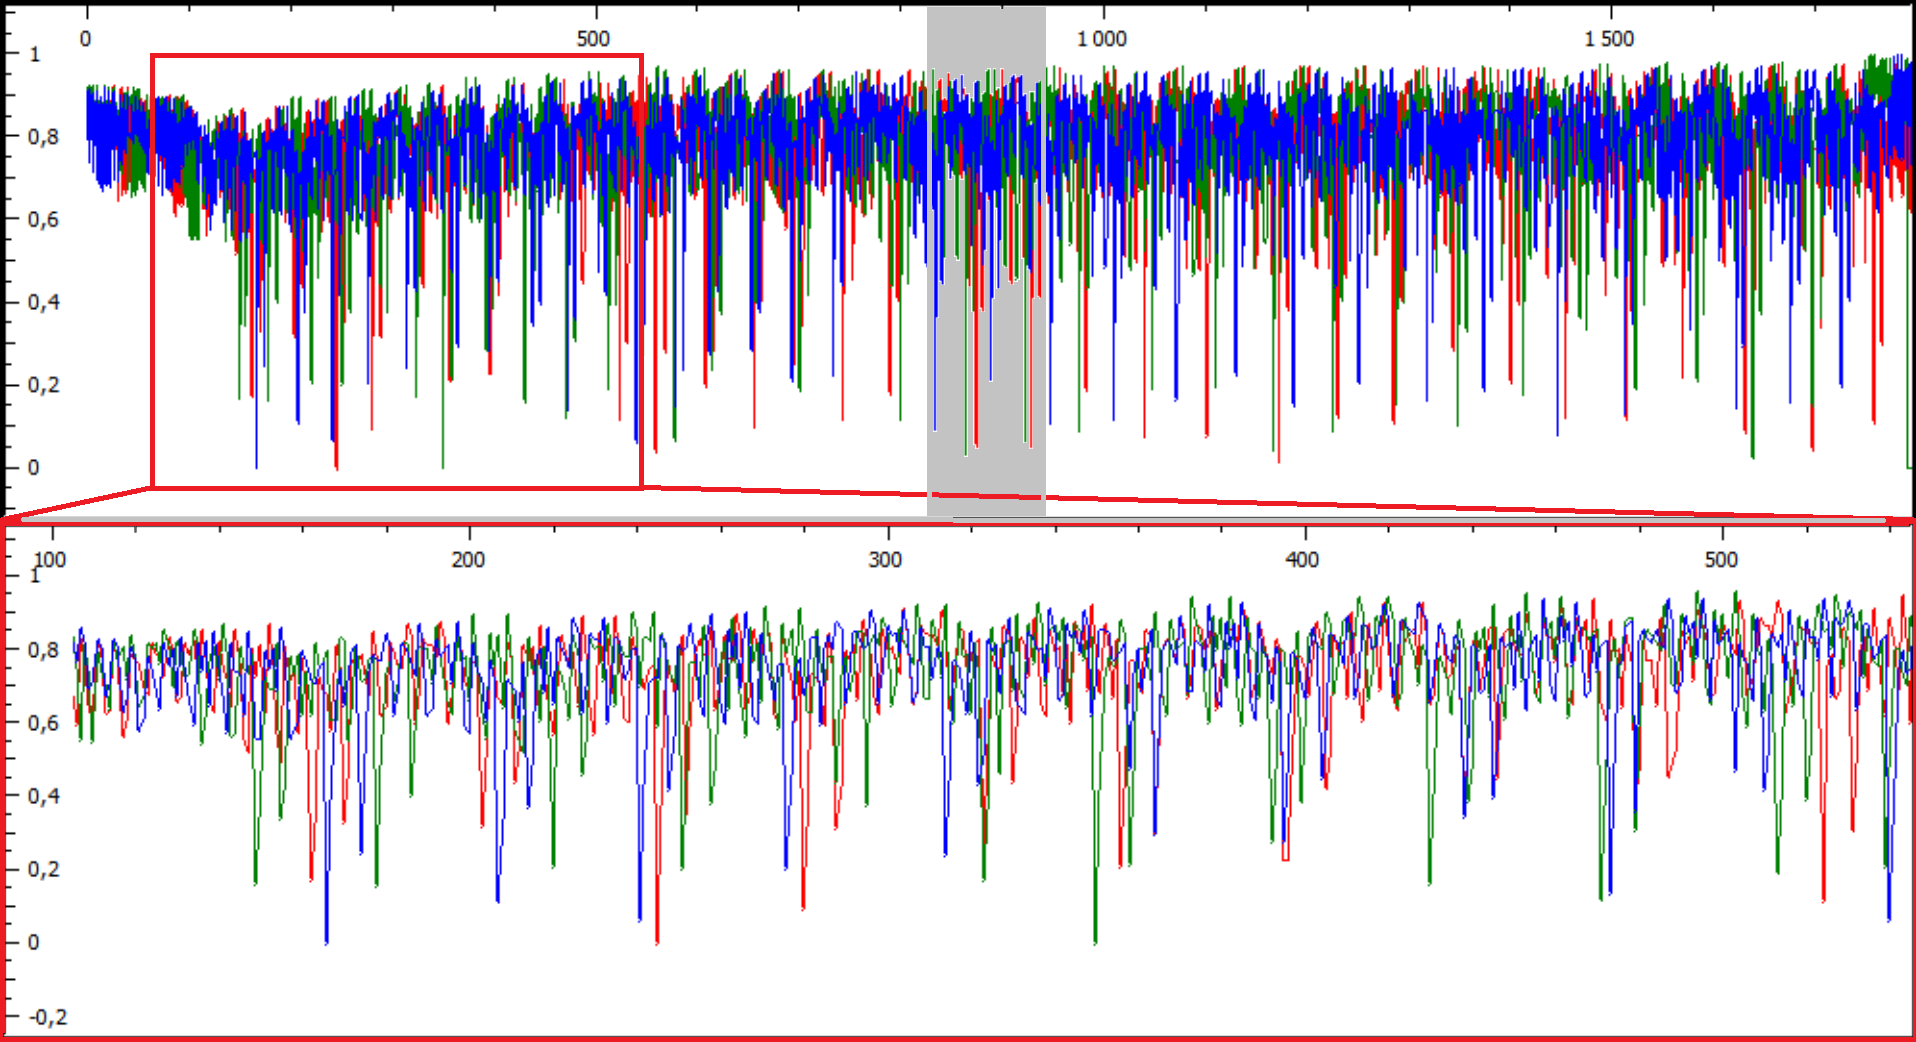
\includegraphics[width=.4\textwidth]{../Figures/CHES2017/jitter_6_6_framed.png} }
\end{figure}
\begin{block}{Target}

\begin{itemize}
\item Target Variable: $Z = \mathrm{HW}(\mathrm{Sbox}(P\oplus K))$
\item $\approx 2000$ time samples
\item Countermeasure: artificial signal treatment simulating clock jitter
\item 10000 training traces
\end{itemize}
\end{block}


\end{frame}

\begin{frame}
\frametitle{Artificial Jitter (2)}
\vspace*{-10pt}
\begin{scriptsize}
\newcolumntype{C}{>{\centering\arraybackslash}p{3em}}
\begin{table}[t]
\centering

\begin{tabular}{|C|C|CCCCCC|}
\multicolumn{8}{C}{\emph{Low\_jitter}}      \\                                            
\hline
Acc                          & $N^\star$                         & \multicolumn{2}{C|}{$\mathrm{SH}_{0}$}                                                   & \multicolumn{2}{C|}{$\mathrm{SH}_{20}$}                                                & \multicolumn{2}{C|}{$\mathrm{SH}_{40}$}                                           \\ \hline
\multicolumn{2}{|C|}{$\mathrm{AR}_{0}$}   & \multicolumn{1}{C|}{\cellcolor[HTML]{EFEFEF}57.4\%}  & \multicolumn{1}{C|}{\cellcolor[HTML]{EFEFEF}14}     & \multicolumn{1}{C|}{82.5\%}                         & \multicolumn{1}{C|}{6}                              & \multicolumn{1}{C|}{83.6\%}                                  & 6                                                            \\ \cline{1-8}
\multicolumn{2}{|C|}{$\mathrm{AR}_{100}$} & \multicolumn{1}{C|}{86.0\%}                          & \multicolumn{1}{C|}{6}                              & \multicolumn{1}{C|}{87.0\%}                         & \multicolumn{1}{C|}{5}                              & \multicolumn{1}{C|}{87.5\%}                                  & 6                                                             \\ \cline{1-8}
\multicolumn{2}{|C|}{$\mathrm{AR}_{200}$} & \multicolumn{1}{C|}{86.6\%}                          & \multicolumn{1}{C|}{6}                              & \multicolumn{1}{C|}{85.7\%} & \multicolumn{1}{C|}{6}      & \multicolumn{1}{C|}{\textbf{87.7\%}} & \textbf{5}      \\ \hline


\end{tabular}


\end{table}
\begin{table}[t]
\centering


\begin{tabular}{|C|C|CCCCCC|}
\multicolumn{8}{C}{\emph{High\_jitter}}      \\   
\hline
Acc                          & $N^\star$                         & \multicolumn{2}{C|}{$\mathrm{SH}_{0}$}                                                   & \multicolumn{2}{C|}{$\mathrm{SH}_{20}$}                                              & \multicolumn{2}{C|}{$\mathrm{SH}_{40}$}                                             \\ \hline
\multicolumn{2}{|C|}{$\mathrm{AR}_{0}$}   & \multicolumn{1}{C|}{\cellcolor[HTML]{EFEFEF}40.6\%} & \multicolumn{1}{C|}{\cellcolor[HTML]{EFEFEF}35}  & \multicolumn{1}{C|}{51.1\%} & \multicolumn{1}{C|}{9}      & \multicolumn{1}{C|}{62.4\%}           & 11                                 \\ \cline{1-8}
\multicolumn{2}{|C|}{$\mathrm{AR}_{100}$} & \multicolumn{1}{C|}{50.2\%} & \multicolumn{1}{C|}{15}     & \multicolumn{1}{C|}{72.4\%} & \multicolumn{1}{C|}{11}     & \multicolumn{1}{C|}{73.5\%}           & 9                       \\ \cline{1-8}
\multicolumn{2}{|C|}{$\mathrm{AR}_{200}$} & \multicolumn{1}{C|}{64.0\%} & \multicolumn{1}{C|}{11}     & \multicolumn{1}{C|}{\textbf{75.5\%}} & \multicolumn{1}{C|}{\textbf{8}}   & \multicolumn{1}{C|}{74.4\%}           & 8           \\ \hline


\end{tabular}


\end{table}
\end{scriptsize}


\begin{figure}
\subfloat[Low Jitter]{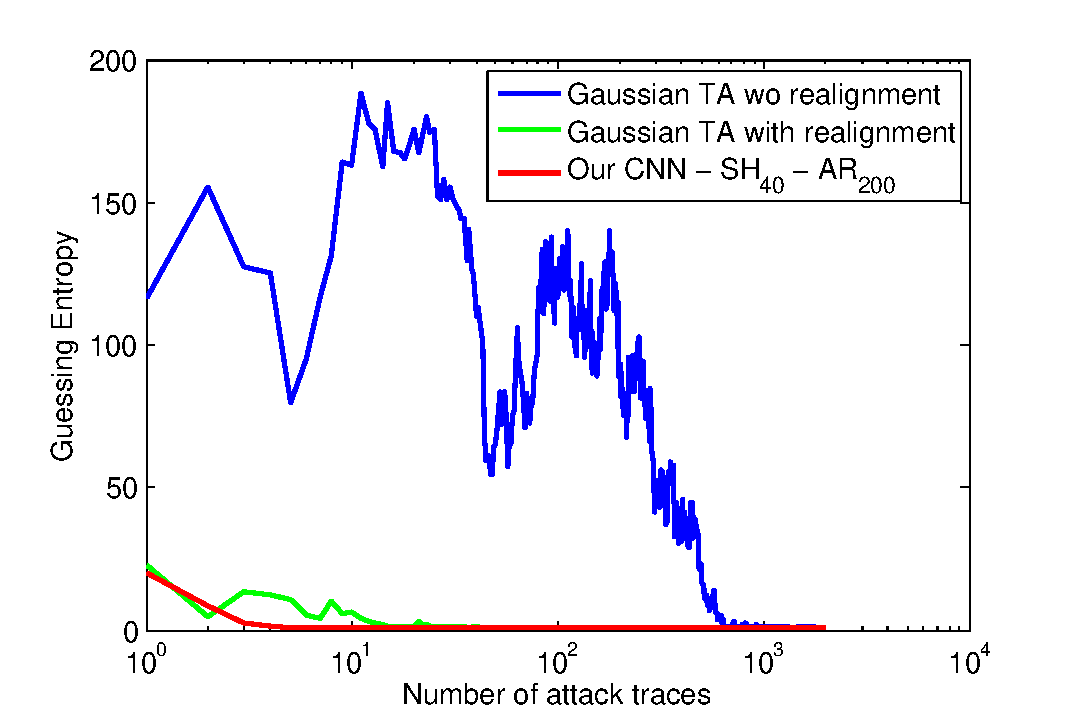
\includegraphics[width=.45\textwidth]{../Figures/CHES2017/results_low_jitter_new.pdf} }
\subfloat[High Jitter]{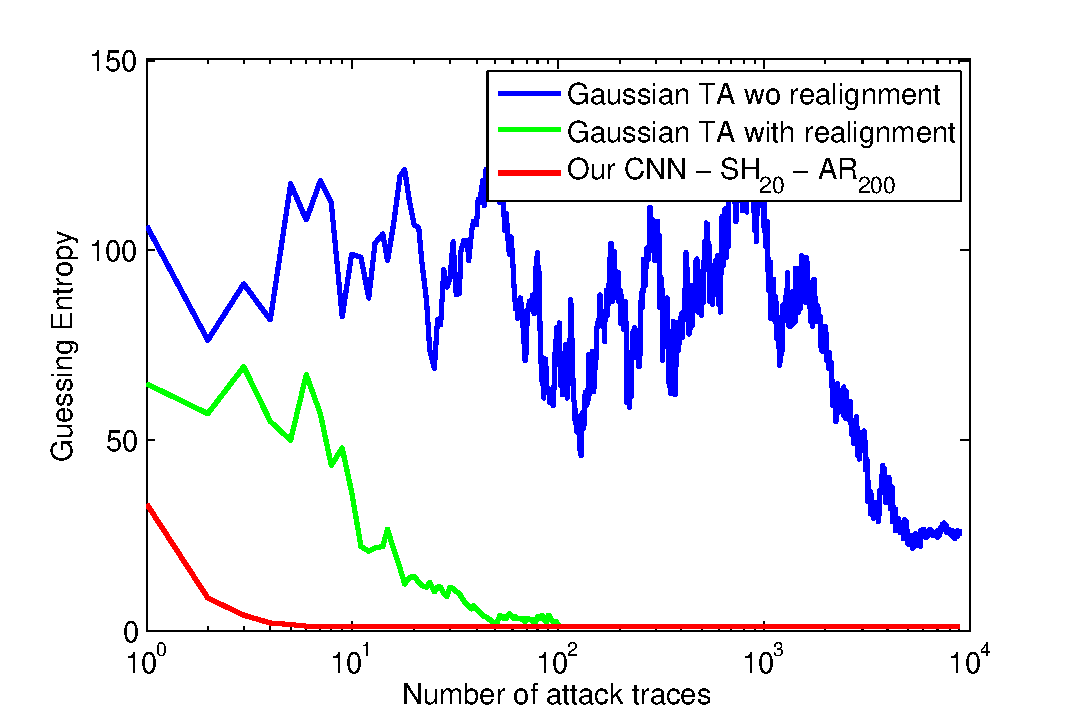
\includegraphics[width=.45\textwidth]{../Figures/CHES2017/results_high_jitter_new.pdf} }

\end{figure}
\end{frame}



\begin{frame}
\frametitle{Artificial Jitter}
\begin{tiny}

\newcolumntype{C}{>{\centering\arraybackslash}p{3em}}
\begin{table}[t]
\centering
\label{table:results_all}



\begin{tabular}{|C|C|CCCCCC|CC}
\hline
\multicolumn{10}{|C|}{\textbf{\emph{DS\_low\_jitter}}}\\
\hline
$a$                           & $b$                         & \multicolumn{2}{C|}{}                                                                                      & \multicolumn{2}{C|}{}                                                                                     & \multicolumn{2}{C|}{}                                                                                  & \multicolumn{2}{C|}{}                                      \\ \cline{1-2}
$c$                           & $d$                         & \multicolumn{2}{C|}{\multirow{-2}{*}{$\mathrm{SH}_{0}$}}                                                   & \multicolumn{2}{c|}{\multirow{-2}{*}{$\mathrm{SH}_{20}$}}                                                 & \multicolumn{2}{c|}{\multirow{-2}{*}{$\mathrm{SH}_{40}$}}                                              & \multicolumn{2}{c|}{\multirow{-2}{*}{$\mathrm{SH}_{200}$}} \\ \hline
\multicolumn{2}{|c|}{}                                      & \multicolumn{1}{c|}{\cellcolor[HTML]{EFEFEF}100.0\%} & \multicolumn{1}{c|}{\cellcolor[HTML]{EFEFEF}68.7\%} & \multicolumn{1}{c|}{99.8\%}                         & \multicolumn{1}{c|}{86.1\%}                         & \multicolumn{1}{c|}{98.9\%}                                  & 84.1\%                                  &                              &                             \\ \cline{3-8}
\multicolumn{2}{|c|}{\multirow{-2}{*}{$\mathrm{AR}_{0}$}}   & \multicolumn{1}{c|}{\cellcolor[HTML]{EFEFEF}57.4\%}  & \multicolumn{1}{c|}{\cellcolor[HTML]{EFEFEF}14}     & \multicolumn{1}{c|}{82.5\%}                         & \multicolumn{1}{c|}{6}                              & \multicolumn{1}{c|}{83.6\%}                                  & 6                                       &                              &                             \\ \cline{1-8}
\multicolumn{2}{|c|}{}                                      & \multicolumn{1}{c|}{87.7\%}                          & \multicolumn{1}{c|}{88.2\%}                         & \multicolumn{1}{c|}{82.4\%}                         & \multicolumn{1}{c|}{88.4\%}                         & \multicolumn{1}{c|}{81.9\%}                                  & 89.6\%                                  &                              &                             \\ \cline{3-8}
\multicolumn{2}{|c|}{\multirow{-2}{*}{$\mathrm{AR}_{100}$}} & \multicolumn{1}{c|}{86.0\%}                          & \multicolumn{1}{c|}{6}                              & \multicolumn{1}{c|}{87.0\%}                         & \multicolumn{1}{c|}{5}                              & \multicolumn{1}{c|}{87.5\%}                                  & 6                                       &                              &                             \\ \cline{1-8}
\multicolumn{2}{|c|}{}                                      & \multicolumn{1}{c|}{83.2\%}                          & \multicolumn{1}{c|}{88.6\%}                         & \multicolumn{1}{c|}{81.4\%} & \multicolumn{1}{c|}{86.9\%} & \multicolumn{1}{c|}{\textbf{80.6\%}} &\textbf{88.9\%} &                              &                             \\ \cline{3-8}
\multicolumn{2}{|c|}{\multirow{-2}{*}{$\mathrm{AR}_{200}$}} & \multicolumn{1}{c|}{86.6\%}                          & \multicolumn{1}{c|}{6}                              & \multicolumn{1}{c|}{85.7\%} & \multicolumn{1}{c|}{6}      & \multicolumn{1}{c|}{\textbf{87.7\%}} & \textbf{5}      &                              &                             \\ \hline
\multicolumn{2}{|c|}{}                                      &                                                      &                                                     &                                                     &                                                     &                                                              &                                         & \multicolumn{1}{c|}{85.0\%}  & \multicolumn{1}{c|}{88.6\%} \\ \cline{9-10} 
\multicolumn{2}{|c|}{\multirow{-2}{*}{$\mathrm{AR}_{500}$}} &                                                      &                                                     &                                                     &                                                     &                                                              &                                         & \multicolumn{1}{c|}{86.2\%}  & \multicolumn{1}{c|}{5}      \\ \cline{1-2} \cline{9-10}
\multicolumn{10}{|C|}{}\\
\hline
\multicolumn{10}{|C|}{\textbf{\emph{DS\_high\_jitter}}}\\
\hline
$a$                          & $b$                         & \multicolumn{2}{C|}{\multirow{2}{*}{$\mathrm{SH}_{0}$}}   & \multicolumn{2}{C|}{\multirow{2}{*}{$\mathrm{SH}_{20}$}}  & \multicolumn{2}{C|}{\multirow{2}{*}{$\mathrm{SH}_{40}$}} & \multicolumn{2}{C|}{\multirow{2}{*}{$\mathrm{SH}_{200}$}} \\ \cline{1-2}
$c$                          & $d$                         & \multicolumn{2}{C|}{}                                     & \multicolumn{2}{C|}{}                                     & \multicolumn{2}{C|}{}                                    & \multicolumn{2}{C|}{}                                     \\ \hline
\multicolumn{2}{|C|}{\multirow{2}{*}{$\mathrm{AR}_{0}$}}   & \multicolumn{1}{C|}{\cellcolor[HTML]{EFEFEF}100\%}  & \multicolumn{1}{l|}{\cellcolor[HTML]{EFEFEF}45.0\%} & \multicolumn{1}{C|}{100\%}  & \multicolumn{1}{C|}{60.0\%} & \multicolumn{1}{l|}{98.5\%}           & 67.6\%           &                             &                             \\ \cline{3-8}
\multicolumn{2}{|C|}{}                                     &  \multicolumn{1}{C|}{\cellcolor[HTML]{EFEFEF}40.6\%} & \multicolumn{1}{C|}{\cellcolor[HTML]{EFEFEF}35}  & \multicolumn{1}{C|}{51.1\%} & \multicolumn{1}{C|}{9}      & \multicolumn{1}{C|}{62.4\%}           & 11               &                             &                             \\ \cline{1-8}
\multicolumn{2}{|C|}{\multirow{2}{*}{$\mathrm{AR}_{100}$}} & \multicolumn{1}{C|}{90.4\%} & \multicolumn{1}{l|}{57.3\%} & \multicolumn{1}{C|}{76.6\%} & \multicolumn{1}{C|}{73.6\%} & \multicolumn{1}{C|}{78.5\%}           & 76.4\%           &                             &                             \\ \cline{3-8}
\multicolumn{2}{|C|}{}                                     & \multicolumn{1}{C|}{50.2\%} & \multicolumn{1}{C|}{15}     & \multicolumn{1}{C|}{72.4\%} & \multicolumn{1}{C|}{11}     & \multicolumn{1}{C|}{73.5\%}           & 9                &                             &                             \\ \cline{1-8}
\multicolumn{2}{|C|}{\multirow{2}{*}{$\mathrm{AR}_{200}$}} & \multicolumn{1}{C|}{83.1\%} & \multicolumn{1}{C|}{67.7\%} &\multicolumn{1}{C|}{\textbf{82.0\%}} & \multicolumn{1}{C|}{\textbf{77.1\%}} & \multicolumn{1}{l|}{82.6\%}           & 77.0\%           &                             &                             \\ \cline{3-8}
\multicolumn{2}{|C|}{}                                     & \multicolumn{1}{C|}{64.0\%} & \multicolumn{1}{C|}{11}     & \multicolumn{1}{C|}{\textbf{75.5\%}} & \multicolumn{1}{C|}{\textbf{8}}   & \multicolumn{1}{C|}{74.4\%}           & 8                &                             &                             \\ \hline
\multicolumn{2}{|C|}{\multirow{2}{*}{$\mathrm{AR}_{500}$}} &                             &                             &                             &                             &                                       &                  & \multicolumn{1}{C|}{83.6\%} & \multicolumn{1}{C|}{73.4\%} \\ \cline{9-10} 
\multicolumn{2}{|C|}{}                                     &                             &                             &                             &                             &                                       &                  & \multicolumn{1}{C|}{68.2\%} & \multicolumn{1}{C|}{11}     \\ \cline{1-2} \cline{9-10}  
\end{tabular}


\end{table}

\end{tiny}
\end{frame}

\begin{frame}
\frametitle{Real Jitter (1)}
\vspace{-10pt}
\begin{block}{Target}
\begin{itemize}
\item AES hardware implementation
\item strong jitter effect
\item Target Variable: $Z = \mathrm{Sbox}(P\oplus K)$
\item $2,500$ selected time samples
\item $99,000$ training traces
\end{itemize}
\end{block}

\only<1>{
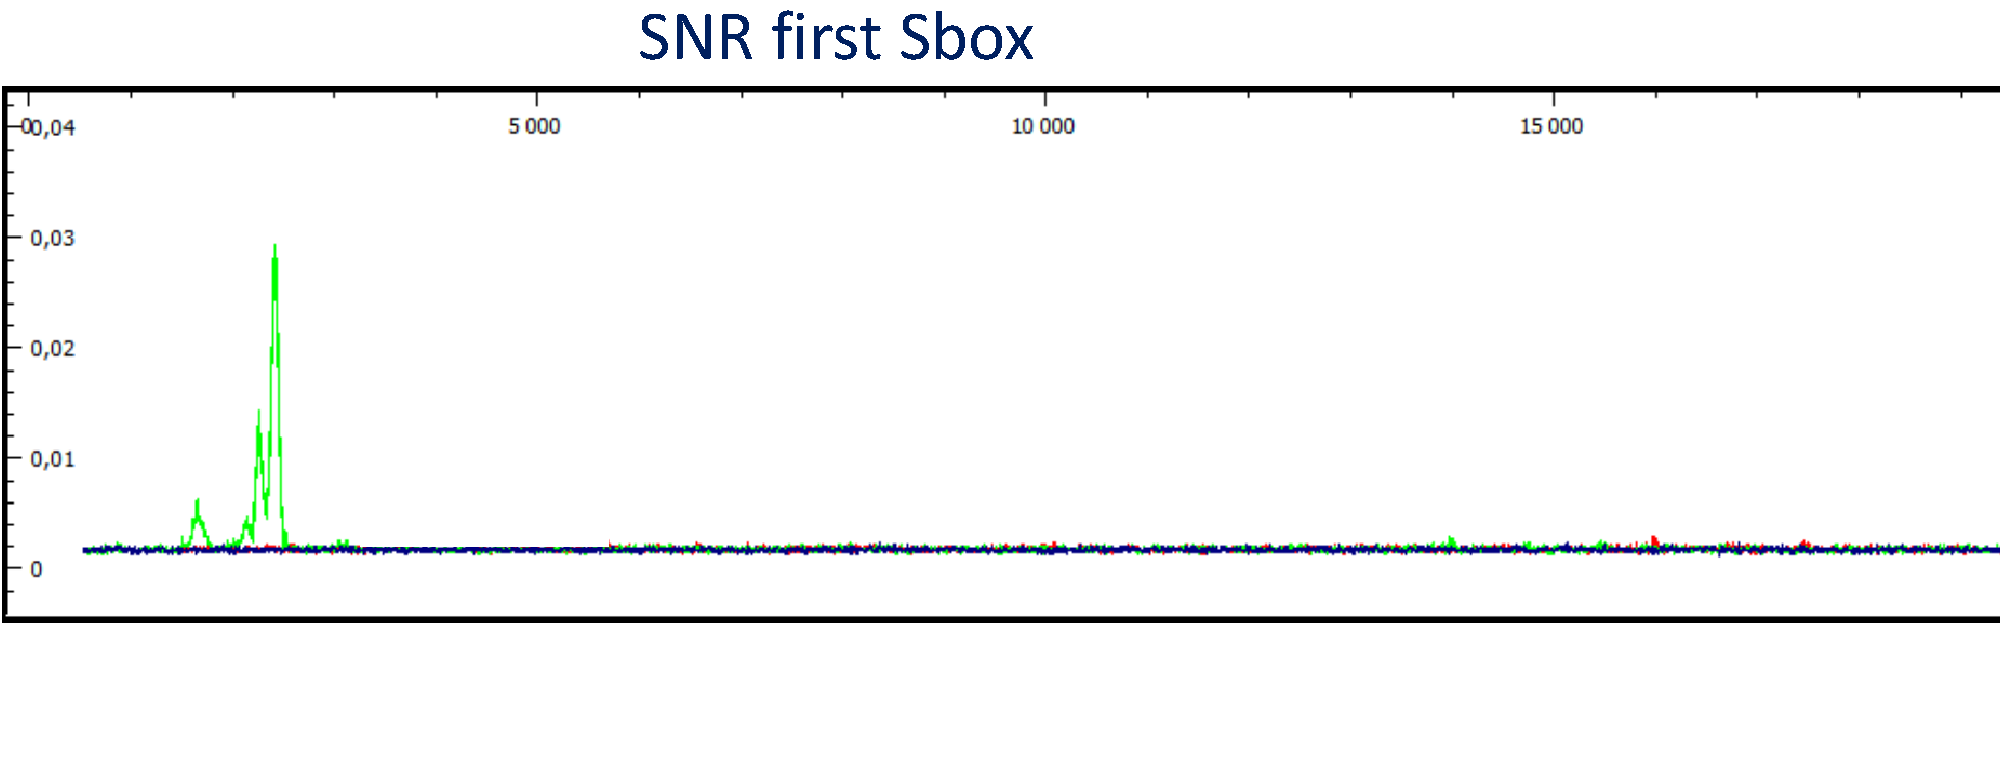
\includegraphics[width=\textwidth]{../Figures/CHES2017/SNR_firstSbox.pdf}
}
\only<2>{
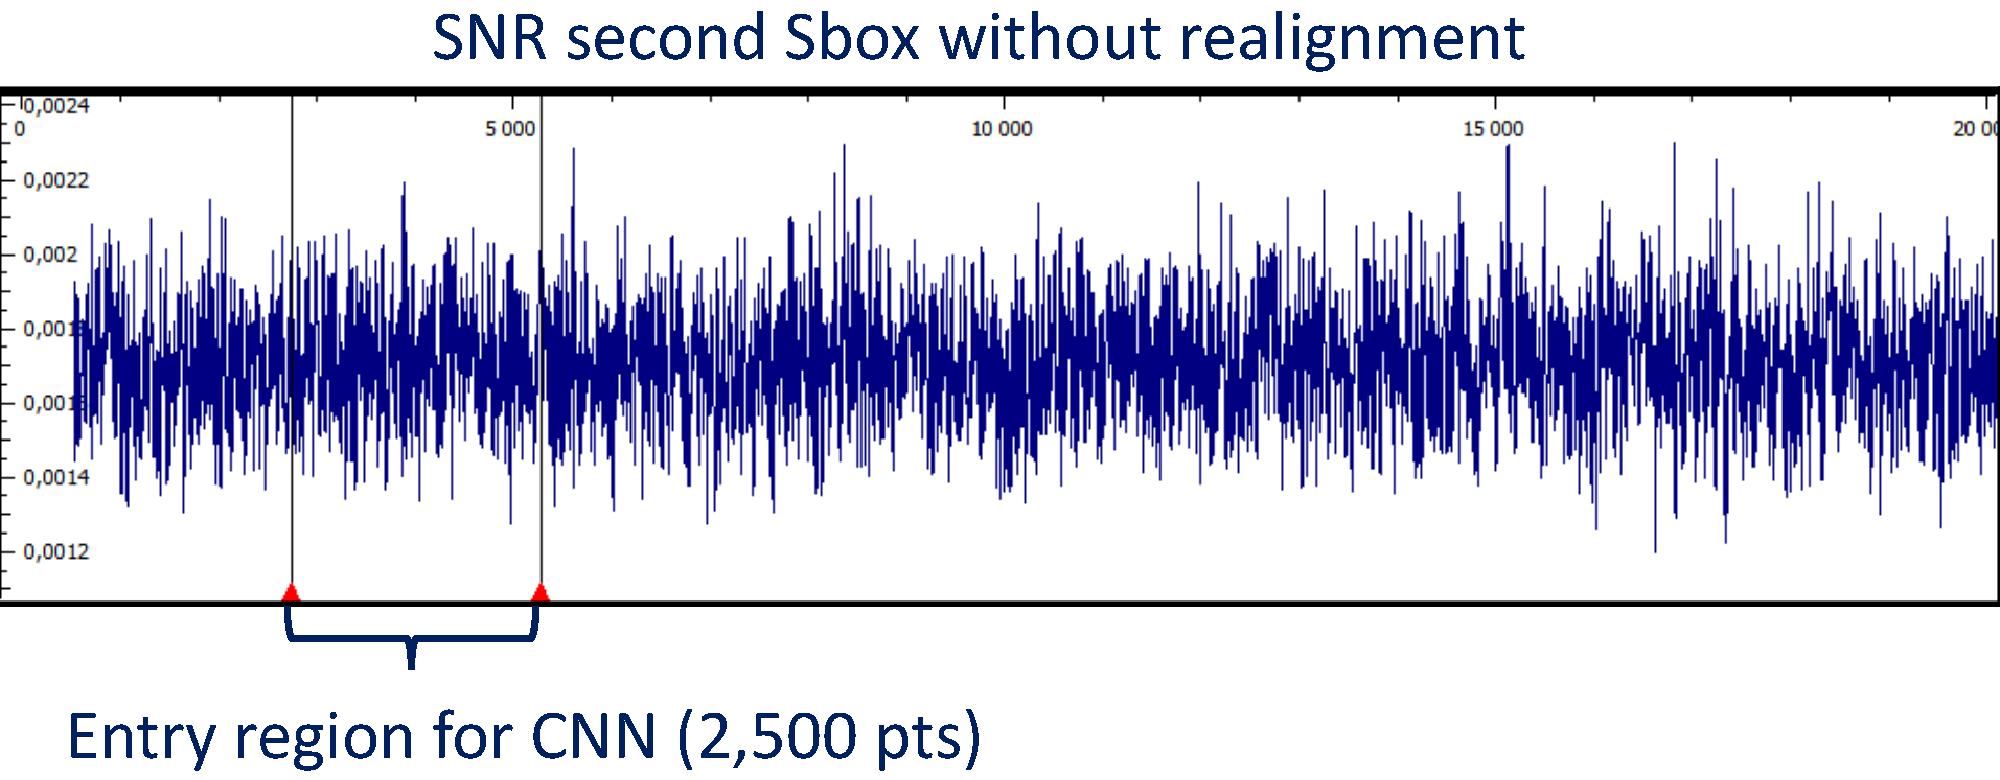
\includegraphics[width=\textwidth]{../Figures/CHES2017/SNR_desynchro.pdf}
}



\end{frame}

\begin{frame}
\frametitle{Real Jitter (2)}
\centering
\begin{scriptsize}
\begin{table}
\begin{tabular}{|c|c|c|c|c|c|c|c|}
\multicolumn{8}{c}{}\\
\hline
\multicolumn{2}{|c|}{} & \multicolumn{2}{c|}{\textcolor{green}{$\mathrm{SH}_{0}$}\textcolor{blue}{$\mathrm{AR}_{0}$}} & \multicolumn{2}{c|}{\textcolor{green}{$\mathrm{SH}_{10}$}\textcolor{blue}{$\mathrm{AR}_{100}$}} & \multicolumn{2}{c|}{\textcolor{green}{$\mathrm{SH}_{20}$}\textcolor{blue}{$\mathrm{AR}_{200}$}} \\ \hline
Acc        & $N^\star$       & 1.2\%                      & 137                      & 1.3\%                       & 89                         & \textbf{1.8\%}              & \textbf{54}                \\ \hline
\end{tabular}
\end{table}
\end{scriptsize}
\uncover<2>{
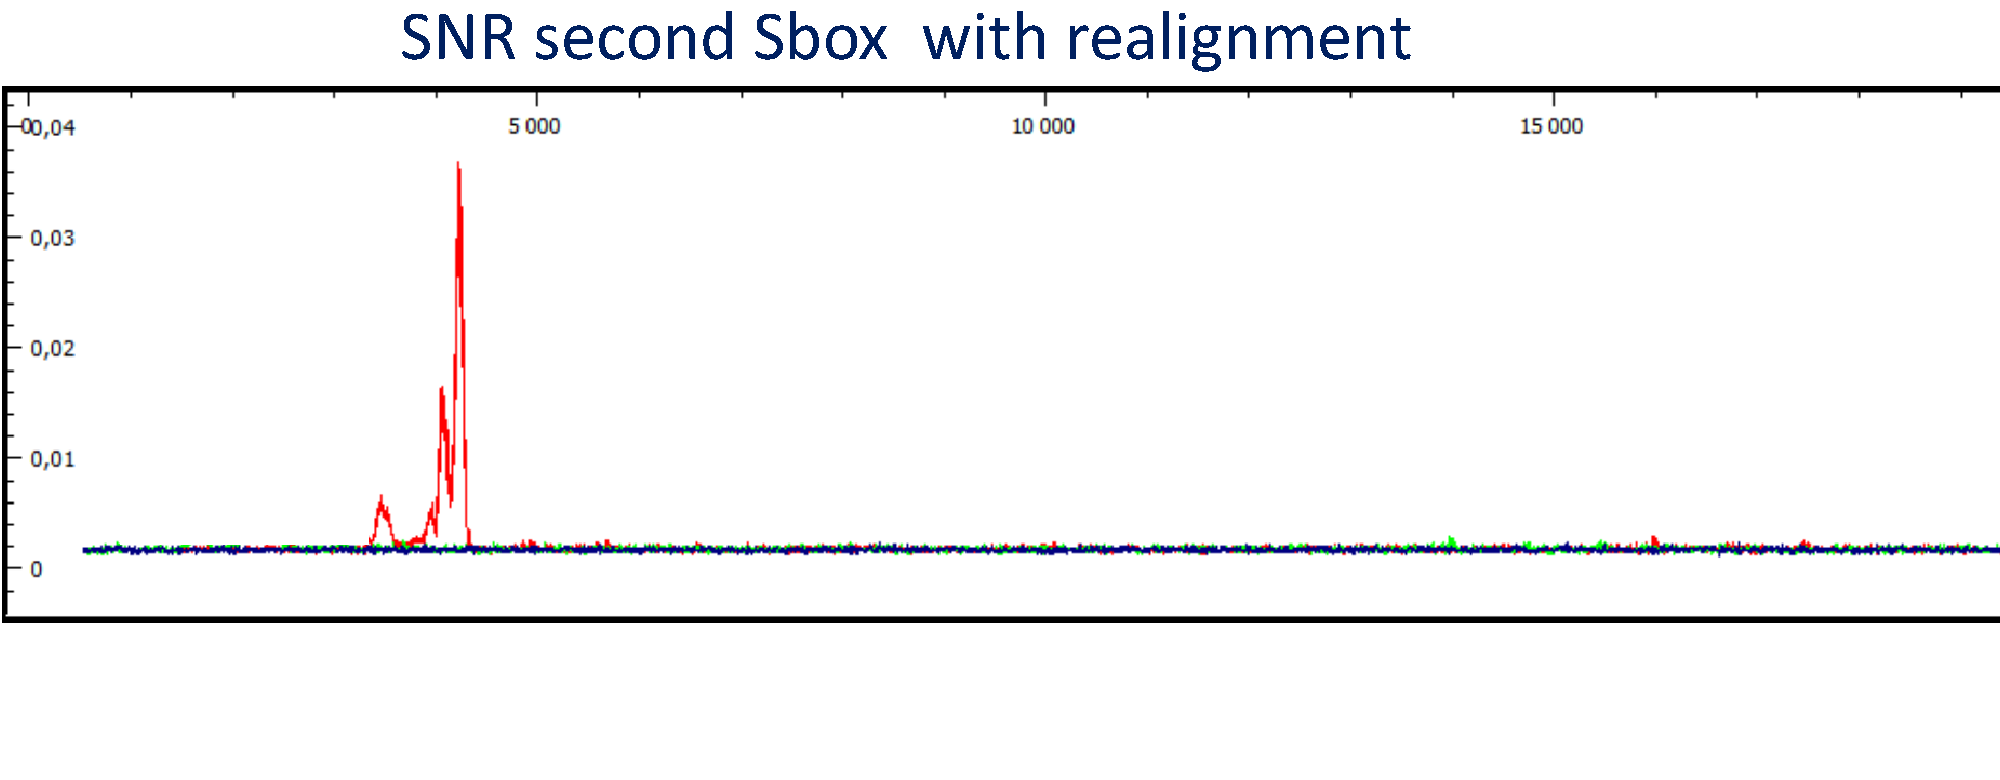
\includegraphics[width=0.75\textwidth]{../Figures/CHES2017/SNR_resynchro.pdf} 
}
\vspace*{-18pt}

\centering
\uncover<2>{
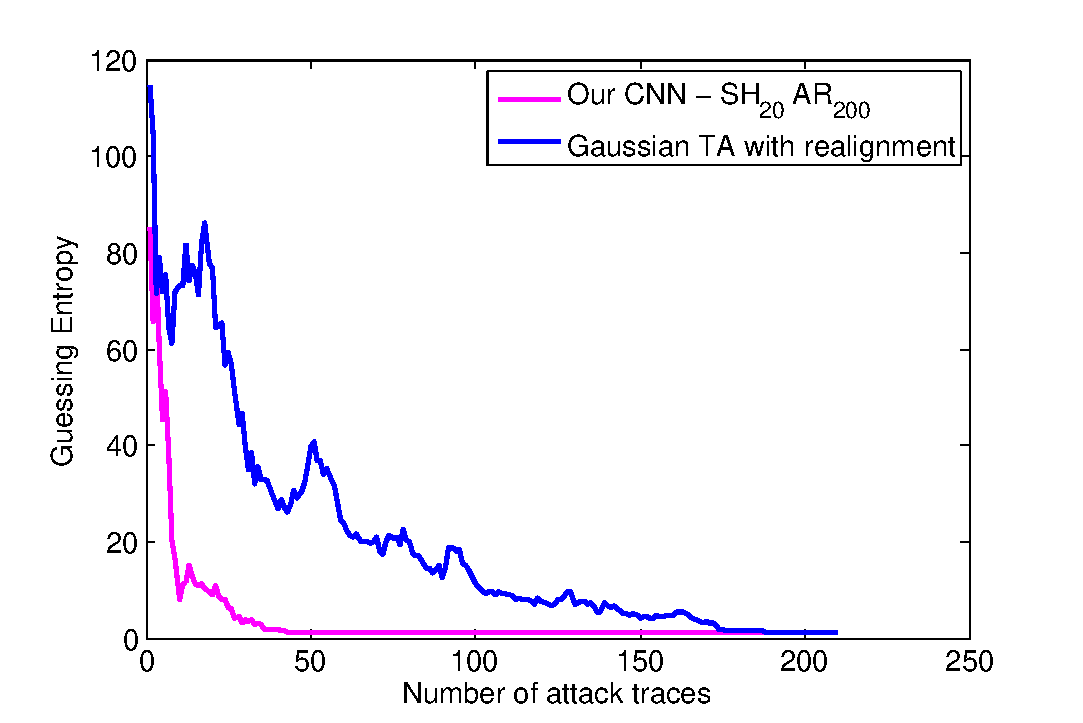
\includegraphics[width=0.5\textwidth]{../Figures/CHES2017/TA_CNN_smartcard.pdf} 
}


\end{frame}
